% Drawing 80/02-7 -- folder 80, batch 02, archive page 24 (PDF page 25).
% Transcription: au-dessous de $\mathrm{IV}_7$, un dessin : sept droites, quatre en trait plein (un quadrilatère complet, ses six sommets marqués en noir) et trois en tirets (les diagonales) ; les trois points de rencontre des diagonales sont entourés d'un petit cercle, celui de droite étant de plus marqué en noir
% Kind: complete quadrilateral with its three diagonals, diagonal points ringed. Method 2 (schematic redraw from the facsimile). Status: ok.
% Notes: Ink. Four solid lines through the six marked vertices; three dashed diagonals, drawn as slightly curved lines through their two vertices and through the three diagonal points as placed on the page (he draws them free-hand; straight lines through the vertices would put the right-hand diagonal point further out). The three diagonal points are ringed, the right one also filled, as on the page (the transcription's note counts two ringed points). The solid end of the horizontal diagonal and the short solid stroke at the lower right are drawn. Redrawn 2026-11-12 (issue 128): to check again.
% Coordinates: 1 unit = 1 mm = 1/100 of the crop width (bbox in page fractions: [0.32, 0.4, 0.68, 0.55]).
% Redrawn by Claude (claude-fable-5-2), issue #128, 2026-11-12; not checked by a human; not compiled (no TeX in the session).
% Rights: reproduces part of the work -- behind RENDER_TRANSCRIPTS, never published by itself.
\documentclass[tikz,border=3pt]{standalone}
\usepackage{amsmath,amssymb}
\usetikzlibrary{patterns,arrows.meta}
\tikzset{pencil/.style={black!45}, struck/.style={black!35}, mpt/.style={circle,draw,inner sep=1.3pt}, pt/.style={circle,fill,inner sep=0.9pt}, opt/.style={circle,draw,fill=white,inner sep=1.1pt}}
\begin{document}
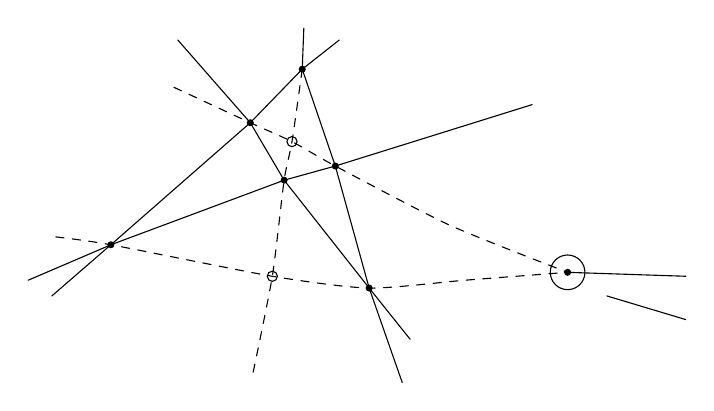
\begin{tikzpicture}[x=1mm,y=1mm,line cap=round,line join=round,font=\scriptsize]
\draw (7.5,-48) -- (15,-41.5) -- (32.7,-26) -- (39.3,-19.2) -- (44,-15.5);
\draw (4.5,-46) -- (15,-41.5) -- (37,-33.3) -- (43.5,-31.5) -- (68.5,-23.7);
\draw (23.5,-15.5) -- (32.7,-26) -- (37,-33.3) -- (47.8,-47) -- (53,-53.5);
\draw (39.5,-14) -- (39.3,-19.2) -- (43.5,-31.5) -- (47.8,-47) -- (52,-59);
\draw[dashed] plot[smooth, tension=0.4] coordinates {(23,-21.5) (32.7,-26) (38,-28.4) (43.5,-31.5) (58,-39) (73,-45)};
\draw (78,-48) -- (88,-51);
\draw[dashed] plot[smooth, tension=0.4] coordinates {(39.3,-19.2) (38,-28.4) (37,-33.3) (35.5,-45.5) (33,-58)};
\draw[dashed] plot[smooth, tension=0.4] coordinates {(8,-40.5) (15,-41.5) (35.5,-45.5) (47.8,-47) (60,-46) (73,-45)};
\draw (73,-45) -- (88,-45.5);
\node[pt] at (39.3,-19.2) {};
\node[pt] at (32.7,-26) {};
\node[pt] at (43.5,-31.5) {};
\node[pt] at (37,-33.3) {};
\node[pt] at (15,-41.5) {};
\node[pt] at (47.8,-47) {};
\node[pt] at (73,-45) {};
\node[mpt] at (38,-28.4) {};
\node[mpt] at (35.5,-45.5) {};
\draw (73,-45) circle[radius=2.2];
\end{tikzpicture}
\end{document}
